% !TeX root = ../main.tex

% Edit this title for each week's entry.
\section{Week 3 - Financial Instruments}

\topic{Mortgages}

\begin{definition}[Mortgage]
    A loan secured by \textbf{real property}: you borrow money and use the
    property as collateral. From French law, ``death contract'' (\emph{mort-}
    = death): the pledge ends when the obligation is fulfilled.
\end{definition}

\heading{Importance of Mortgages}
\begin{itemize}
    \item The most common way to finance a home: new purchases with a mortgage outnumber those without by a factor of 6 (CMHC)
    \item Mortgages are by far the largest share of Canadian household debt
\end{itemize}
\begin{center}
    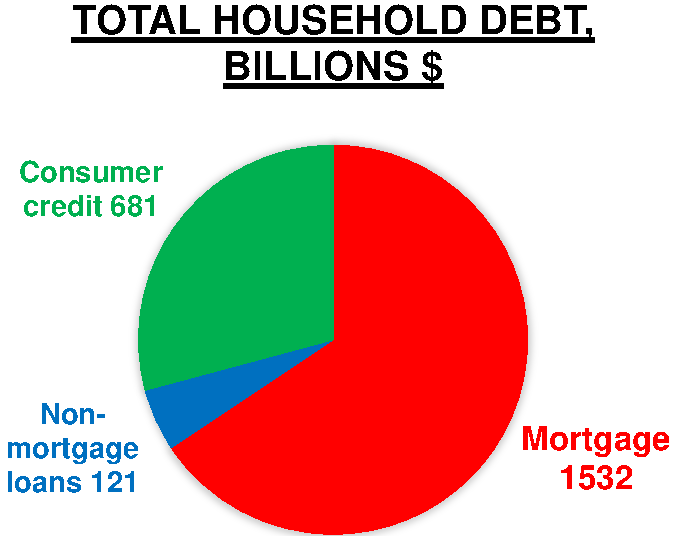
\includegraphics[width=0.35\linewidth]{figures/household_debt_pie.png}
    \\[2pt] \textit{\small Total household debt, billions \$ (Statistics Canada)}
\end{center}

\heading{Mortgage Terminology}
Buying a \$500,000 house:
\begin{itemize}
    \item \rb{Principal}: the amount you borrow, up to some fraction of the price (e.g.\ 80\% $\Rightarrow$ \$400,000)
    \item \rb{Down payment}: the rest, which you pay yourself (\$100,000)
    \item \rb{Loan-to-value ratio (LTV)}: mortgage loan / value of house $= 400{,}000/500{,}000 = 0.8$
    \item \rb{Mortgage rate}: the interest rate the bank charges on the principal (e.g.\ 5\%/year)
    \item \rb{Amortization period}: the agreed time horizon for full repayment (e.g.\ 25 years)
    \item \rb{Term}: the shorter period over which the agreed rate is fixed (e.g.\ 5 years). After the term ends, the rate is renegotiated and the payments may change
\end{itemize}

\begin{remark}
    Payments are calculated based on the \textbf{amortization period},
    \textbf{not} the term! Canadian mortgage rates are quoted as nominal
    annual rates with \textbf{semi-annual compounding}, so convert to the
    equivalent monthly rate before using $(A/P,i,N)$.
\end{remark}

\begin{example}[Mortgage Payments Across Terms]
    A \$500,000 home with a 20\% down payment. The mortgage rate is 5\%,
    with a 5-year term and a 25-year amortization period.
    \begin{enumerate}[label = \alph*)]
        \item What is the monthly payment during this term?
        \\\db{Principal $P = 0.8(500{,}000) = \$400{,}000$. Semi-annual rate $2.5\%$, so the monthly rate satisfies $(1+i_m)^6 = 1.025$:}
        \[i_m = 1.025^{1/6} - 1 = 0.41239\%, \qquad N = 25 \times 12 = 300\]
        \[A = 400{,}000(A/P,0.41239\%,300) = \db{\$2{,}326.42 \text{ per month}}\]
        \item After the term, the new mortgage rate is 6\%. What is the new monthly payment?
        \\\db{The amount still owed after 60 payments is the PV of the 240 remaining payments at the old rate:}
        \[B_{60} = 2{,}326.42(P/A,0.41239\%,240) = \$354{,}030\]
        \db{Re-amortize this over the remaining 20 years at the new rate, $i_m' = 1.03^{1/6} - 1 = 0.49386\%$:}
        \[A' = 354{,}030(A/P,0.49386\%,240) = \db{\$2{,}521.36 \text{ per month}}\]
    \end{enumerate}
\end{example}

\begin{center}
    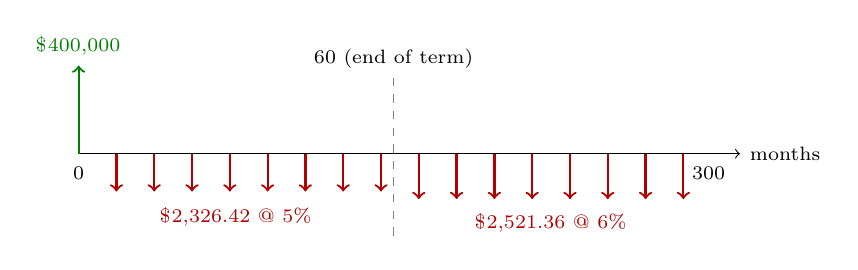
\begin{tikzpicture}[scale=0.8]
        \draw[->] (0,0) -- (10.5,0) node[right] {\scriptsize months};
        \draw[->,thick,green!50!black] (0,0) -- (0,1.4) node[above] {\scriptsize \$400,000};
        \foreach \x in {0.6,1.2,...,4.9}{\draw[->,thick,red!70!black] (\x,0) -- (\x,-0.6);}
        \foreach \x in {5.4,6.0,...,9.9}{\draw[->,thick,red!70!black] (\x,0) -- (\x,-0.72);}
        \draw[dashed,gray] (5,-1.3) -- (5,1.2);
        \node[below] at (0,-0.05) {\scriptsize 0};
        \node[above] at (5,1.2) {\scriptsize 60 (end of term)};
        \node[below] at (10,-0.05) {\scriptsize 300};
        \node[red!70!black] at (2.5,-1.0) {\scriptsize \$2,326.42 @ 5\%};
        \node[red!70!black] at (7.5,-1.1) {\scriptsize \$2,521.36 @ 6\%};
    \end{tikzpicture}
    \\[2pt] \textit{\small Borrower's view: payments step up at the renewal}
\end{center}

\heading{Some Canadian Mortgage Rules}
\begin{itemize}
    \item Since 2012, amortization periods of up to 25 years are allowed
    \item For 25-year amortization, the down payment must be at least 20\%
    \item For shorter amortization periods, the down payment may be smaller ($<20\%$), but \b{mortgage insurance} is required
    \item Real-life mortgages can be more complicated: rates can be variable within a term, you can pay the mortgage down faster, \dots
\end{itemize}

\heading{Summary}
\begin{enumerate}
    \item Mortgages are loans backed by real property (the most common way to finance a home)
    \item Payments are calculated from the principal, mortgage rate, and \b{amortization period}
    \item At the end of each term, the next payments are set by the \b{amount still owed}, the \b{new rate}, and the \b{remaining amortization period}
\end{enumerate}

\topic{Bonds}

\begin{definition}[Bond]
    A financial instrument issued by firms and governments (federal,
    provincial, municipal) to raise funds for projects. It is a special form
    of loan, usually long-term (up to 30 years). The issuer (the borrower)
    promises to pay:
    \begin{itemize}
        \item a stated amount at specified intervals for a defined period: the \rb{coupon payments}
        \item a final amount at a specific date: the \rb{face value}
    \end{itemize}
    Bonds are usually tradeable at any time.
\end{definition}

\heading{Reading a Bond (Ontario Hydro)}
\begin{itemize}
    \item \rb{Face value}: the amount paid at maturity (\$1,000)
    \item \rb{Maturity date}: when the face value is paid (January 6, 2004)
    \item \rb{Coupon rate}: the (nominal annual) rate used to calculate coupon payments ($9\tfrac14\%$)
    \item \rb{Coupon frequency}: how often coupons are paid (January 6 and July 6, i.e.\ semi-annually)
\end{itemize}
\begin{center}
    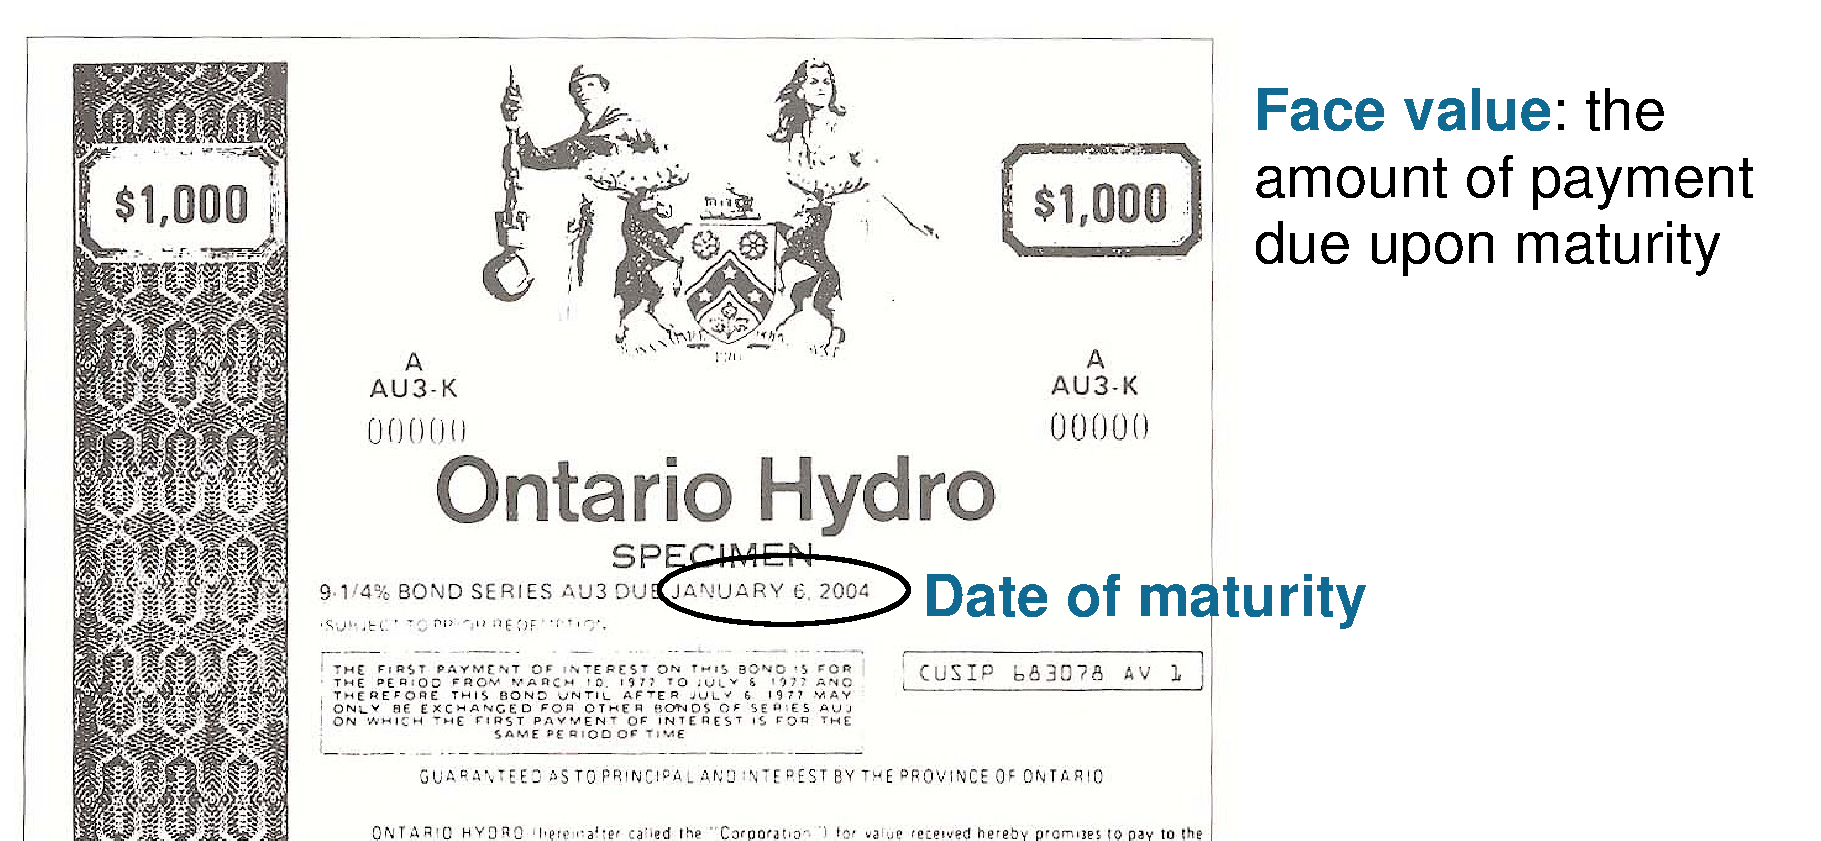
\includegraphics[width=0.62\linewidth]{figures/bond_face_annotated.png}
    \\[4pt]
    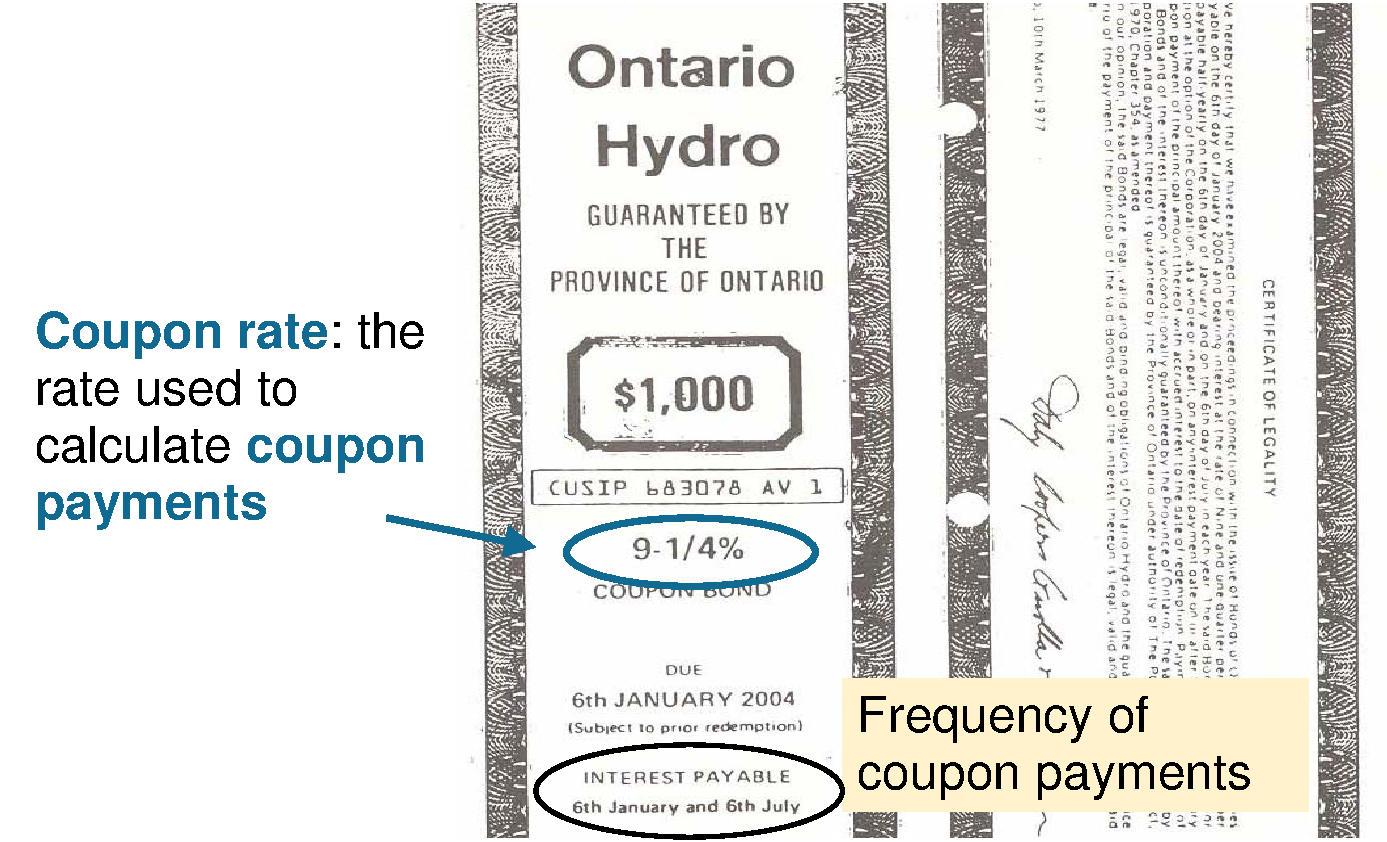
\includegraphics[width=0.5\linewidth]{figures/bond_back_annotated.png}
    \hspace{1em}
    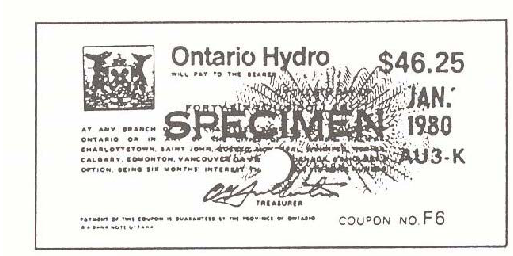
\includegraphics[width=0.3\linewidth]{figures/bond_coupon.png}
\end{center}
\db{Each semi-annual coupon $= 1000 \times 9.25\% / 2 = \$46.25$, matching the coupon shown.}

\heading{Bond Cash-flow Diagram}
From the bondholder's view: pay the price $P$ now, receive coupon $C$ every
period for $N$ periods, plus the face value $F$ at maturity.
\begin{center}
    \begin{tikzpicture}[scale=0.8]
        \draw[->] (0,0) -- (8.5,0) node[right] {\scriptsize $t$};
        \foreach \x in {1,...,7}{\draw[->,thick,green!50!black] (\x,0) -- (\x,0.6);}
        \draw[->,thick,green!50!black] (7,0.6) -- (7,2) node[above] {\scriptsize $F$};
        \node[green!50!black] at (4,0.9) {\scriptsize $C$ each period};
        \draw[->,thick,red!70!black] (0,0) -- (0,-1.2) node[below] {\scriptsize price $P$};
        \node[below] at (7,-0.05) {\scriptsize $N$};
    \end{tikzpicture}
\end{center}
\[\boxed{P = C(P/A,i,N) + F(P/F,i,N)}\]
where $i$ is the yield per coupon period.

\begin{example}[How Much Is This Bond Worth?]
    Ontario Hydro will pay you \$1,000 in 10 years, plus coupons at 9.25\%
    paid every 6 months. If the bank pays 10\% interest, what amount must be
    deposited now to produce the same cash-flows?
    \\\db{$C = \$46.25$, $N = 20$ half-years, $i = 10\%/2 = 5\%$ per half-year:}
    \begin{align*}
        P &= 46.25(P/A,5\%,20) + 1000(P/F,5\%,20)\\
        &= 46.25(12.4622) + 1000(0.37689) = \db{\$953.27}
    \end{align*}
    Would you be willing to pay \$953?
    \\\db{Only if the bond were as safe as the bank. Ontario Hydro might default, so you should demand a lower price.}
\end{example}

\begin{definition}[Yield]
    Risk == reward: the buyer must be compensated for the risk of default by
    paying a \textbf{lower} price. The \rb{yield} is the (hypothetical)
    interest rate that makes the discounted bond payments equal to the price.
    The yield reflects the time value of money for the bond's payments.
\end{definition}

\begin{example}[Yield from a Price]
    If the highest price you are willing to pay for the bond above is \$700,
    what annual interest rate gives that price?
    \[700 = 46.25(P/A,i,20) + 1000(P/F,i,20)\]
    \db{Solving numerically (trial and error or a solver): $i = 7.587\%$ per half-year, i.e.\ a nominal yield of $\approx 15.2\%$/year (effective $15.75\%$).}
\end{example}

\heading{Bond Price Is Determined by Yield}
\begin{itemize}
    \item Price $=$ payments discounted at the yield, so a higher yield means a lower price
    \item When yield $=$ coupon rate, price $=$ face value (``at par''). When yield $>$ coupon rate, price $<$ face value (``at a discount''), and vice versa
\end{itemize}
\begin{center}
    \begin{tikzpicture}[xscale=0.45, yscale=0.35]
        % y in hundreds of dollars (keeps coordinates within TeX's dimension limit)
        \draw[->] (2,0) -- (21,0) node[right] {\scriptsize yield (\%)};
        \draw[->] (2,0) -- (2,15.5) node[above] {\scriptsize price (\$)};
        \foreach \x in {4,8,12,16,20}{\draw (\x,0.15) -- (\x,-0.15) node[below] {\scriptsize \x};}
        \foreach \y in {5,10,15}{\draw (2.15,\y) -- (1.85,\y) node[left] {\scriptsize \y00};}
        \draw[thick,blue!60!black,domain=3:20,samples=60]
            plot (\x, {0.4625*(1-(1+\x/200)^(-20))/(\x/200) + 10*(1+\x/200)^(-20)});
        \draw[dashed,gray] (2,10) -- (9.25,10) -- (9.25,0);
        \fill (9.25,10) circle (2pt);
        \node[above right] at (9.25,10) {\scriptsize at par (9.25\%)};
        \fill (10,9.5327) circle (2pt);
        \node[right] at (10.2,9.1) {\scriptsize \$953 @ 10\%};
        \fill (15.17,7) circle (2pt);
        \node[right] at (15.4,7) {\scriptsize \$700 @ 15.2\%};
    \end{tikzpicture}
    \\[2pt] \textit{\small Ontario Hydro bond (\$1,000 face, 9.25\% semi-annual coupon, 10 years)}
\end{center}

\begin{example}[Reflection]
    If the bond yield increases, does the price of the bond increase or decrease?
    \\\db{The price \dbb{decreases}: the same payments are discounted at a higher rate.}
\end{example}

\heading{Yield Depends on Risk and Time to Maturity}
\begin{center}
    \begin{minipage}{0.48\linewidth}\centering
        \begin{tabular}{lr}
            \toprule
            Country & 2-yr gov't yield (2019, \%) \\
            \midrule
            Argentina (1 yr) & 32.59 \\
            Brazil & 5.69 \\
            Canada & 1.521 \\
            China & 2.700 \\
            Germany & $-0.828$ \\
            Uganda & 16.000 \\
            Ukraine & 16.97 \\
            United Kingdom & 0.449 \\
            United States & 1.575 \\
            \bottomrule
        \end{tabular}
        \\[2pt] \textit{\small More stable economies $\Rightarrow$ lower yield}
    \end{minipage}
    \hfill
    \begin{minipage}{0.45\linewidth}\centering
        \begin{tabular}{lr}
            \toprule
            Maturity (yrs) & Gov't of Canada yield (\%) \\
            \midrule
            3 & 1.00 \\
            5 & 1.50 \\
            7 & 2.25 \\
            10 & 2.25 \\
            Long (30) & 2.75 \\
            \bottomrule
        \end{tabular}
        \\[2pt] \textit{\small Longer time to maturity $\Rightarrow$ higher yield}
    \end{minipage}
\end{center}
\db{This is the same idea as the Week 1 interest-rate factors: yield rises with credit (default) risk and maturity risk.}

\heading{Summary}
\begin{enumerate}
    \item \b{Face value, coupon payments/rate, and maturity} are defined by the bond itself
    \item The \rb{yield} is determined by the market (how risky the investment is, interest rate expectations)
    \item Bond prices are calculated by discounting the payments at the bond yield
\end{enumerate}

\topic{Bond Examples}

\begin{example}[Bond Price]
    A \$10,000 bond maturing in 8 years has a 12\% coupon payable quarterly.
    If the yield is 10\%, how much would you pay for the bond?
    \\\db{$C = 10{,}000 \times 12\%/4 = \$300$ per quarter, $N = 32$ quarters, $i = 10\%/4 = 2.5\%$ per quarter:}
    \begin{align*}
        P &= 300(P/A,2.5\%,32) + 10{,}000(P/F,2.5\%,32)\\
        &= 300(21.8492) + 10{,}000(0.45377) = \db{\$11{,}092.46}
    \end{align*}
    \db{Price $>$ face value, because the coupon rate (12\%) exceeds the yield (10\%).}
\end{example}

\begin{example}[Yield on a Bond]
    You buy a bond for \$1,000. The issuer pays a \$45 coupon every 6 months
    and a face value of \$880 at the end of 2 years. What is the
    \rb{effective annual} yield?
    \\\db{Solve for the semi-annual rate $i$ with $N = 4$:}
    \[1000 = 45(P/A,i,4) + 880(P/F,i,4) \;\Rightarrow\; i = 1.570\% \text{ per half-year}\]
    \[i_e = (1 + 0.01570)^2 - 1 = \db{3.16\%}\]
    \db{The yield is low despite the 9\%/year coupons, because you only get \$880 back on a \$1,000 purchase.}
\end{example}
